\chapter{Modelling of {\prox} spectra}
\protect\label{chapter:modelling}
\lhead{Chapter \ref{chapter:modelling} \emph{Modelling of {\prox} spectra}}

In order to develop and refine the methods for evaluation of the periodicity of the sub-peaks in the {\prox} spectra, a
version of the ``Doppler Tomography of Stars'' (DoTS) modelling software \citep{CCamerondotsa} was used. Although DoTS
was written to recover surface imhomogeneities from time series spectra, here the forward modelling routines were used
to generate synthetic spectra, with some modifications. Specifically, a 3D model of the star was constructed, covered in
a finite number of pixels. The intensity of each pixel can vary from a photospheric value to a value appropriate for
plage. In order to obtain the appropriate photospheric intensity for each pixel at a given rotation phase of the 3D
stellar model,the 4-parameter limb darkening law introduced by Claret from Phoenix model atmospheres \citep{claret00a}
was used for an effective temperature of 3000K. The plage intensities were calculated according to \citet[Section
4.1]{unruh99}, who identified the centre to limb variability from plage regions relative to the photospheric (quiet)
intensity for the Sun. Since no such observations exist for other stars, the same law was adopted with appropriate
facular contrasts for {\ha} wavelengths (see \citet[figs 3 \& 4]{unruh99}).

Since it was desired to simulate the {\ha} line profile, a local intensity profile was assumed for the photosphere and
the plage. For inactive photospheres of \rdwarf s with similar spectral type to {\prox}, {\ha} is not visible (e.g. see
{\ha} profile in \citet[fig. 6]{barnes14} for GJ1061). Hence for the quiet photosphere, a flat continuum was assumed For
active stars, {\ha} possesses a characteristic emission profile with self-absorption, resulting in a double-peaked
profile. Since the \textit{vsini} is probably less than 0.1 km/s for \prox, the local line profile shape for {\ha} was
based on the observed {\prox} line profile since it is unlikely to show rotational broadening. This profile was tuned to
resemble the average {\ha} profile shown in the {\uves} data analysed in \citet{fuhrmeister11}, but symmetric about the
central wavelength. Specifically, a Gaussian profile was used to generate the emission peak and a second Gaussian with
narrow width to represent the central self-absorption as illustrated in Fig. \ref{fig:integregions}.

\begin{figure}[!htbp]
\begin{center}
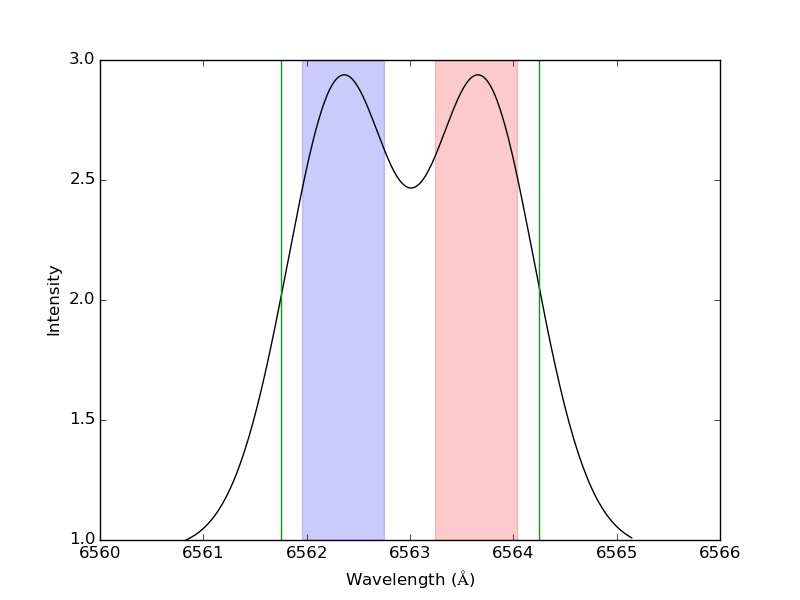
\includegraphics[scale=0.25]{Figures/integregions.png} \\
\end{center}
\caption{Example generated model spectrum of \prox, also illustrating the methods for computing the periodicity of
  spectra.  The centre of the \ha{} line is set at 6563{\AA} for convenience rather than 6562.8\AA{}.  The green lines
  (from 6561.75{\AA} to 6564.25\AA) show the limits used for calculation of the equivalent width. The blue and red
  shaded areas (6561.95{\AA} to 6562.75{\AA} and 6563.44{\AA} to 6564.24{\AA} respectively, each 0.8{\AA} wide) show the
  regions for calculation of the peak ratio.}
\protect\label{fig:integregions}
\end{figure}
% Done with 10 plage 80 period 75 deg first spectrum

With the two-temperature model, in subsequent simulations below, either photospheric intensity or a plage intensity is
assigned to each pixel. For a pixel containing plage, the synthetic {\ha} profile is scaled and for the photosphere with
no visible profile (as note above), the continuum level is used. The line profile is shifted appropriately for the
Doppler shift of each pixel in the model. The model enables the user to place circular spots of specified radii anywhere
on the star. For each viewing angle (or equivalently observation phase), the appropriate intensity profiles of all
visible pixels is calculated (according to position on the line and centre-to-limb variation) and sum them to obtain
the simulated line profile.

A model star with plage regions that rotate into and out of view can thus potentially exhibit variability in the line
shape since the pixels on different parts of the star possess different Doppler velocities. For stars such as \prox,
which probably possess a \textit{vsini} much less than the instrumental resolution, any distortions in the the line
profile due to spots rotating into and out of view may be insignificant or very small. A plage region that rotates into
view may nevertheless have a significant effect on the the equivalent width of the simulated line since the
local intensity profile for {\ha} possesses a normalised peak intensity of N times the continuum. For stars with
rotational velocity much greater than the instrument resolution, line asymmetries are likely to be much more reliable.

\section{Plage distribution and results}
\protect\label{section:plagedists}

During the course of experimentation with models, a selection of plage distributions was tried, ranging from a single
large spot on one face to randomly-placed spots of random sizes. However it was found that the variation in equivalent
widths from a low spot coverage was bore no possible resemblance to that from observational data, in that just exhibited
two extremes of Equivalent Widths and no intermediate values. On the other hand a coverage of more than about 30\%
provided very limited swings in the Equivalent Width compared those observed from {\harps} and {\uves}. After some
experimentation, a randomly distributed plage was settled upon which filled up to 2.5\% of the surface,towards the high
end of the coverage of up to 2.7\% reported in \citet{guttenbrunner14} in relation to the Sun.
% The second was the same combined with a highly fairly asymmetric
% additional 1\% of coverage in a wedge between 0{\degree} and 37{\degree}. To avoid a concentration at the poles the
%likelihood of selecting a latitude point was made to be approximately proportional to the cosine of the latitude.

The models were all generated with the observation dates from the Original Set of {\harps}\footnote{This work was
  completed before the 2016 data was available. Also, as discussed in Section \ref{section:addflares}, it proved useful
  to study the Original Set of data as the 116.6 day period of \citet[Table 3]{suarezmascareno15} appeared in some
  cases.}, using possible rotation periods between 15 and 90 days in steps of 5 days and inclinations between
10{\degree} and 90{\degree} in steps of 5{\degree} to observe the various effects. Only a limited selection, usually
multiples of 10 days and 10{\degree} are shown in this {\paperorthesis} to conserve space.

In Fig. \ref{fig:extremew} some extremes are shown.

\begin{figure}[!htbp]
\begin{center}
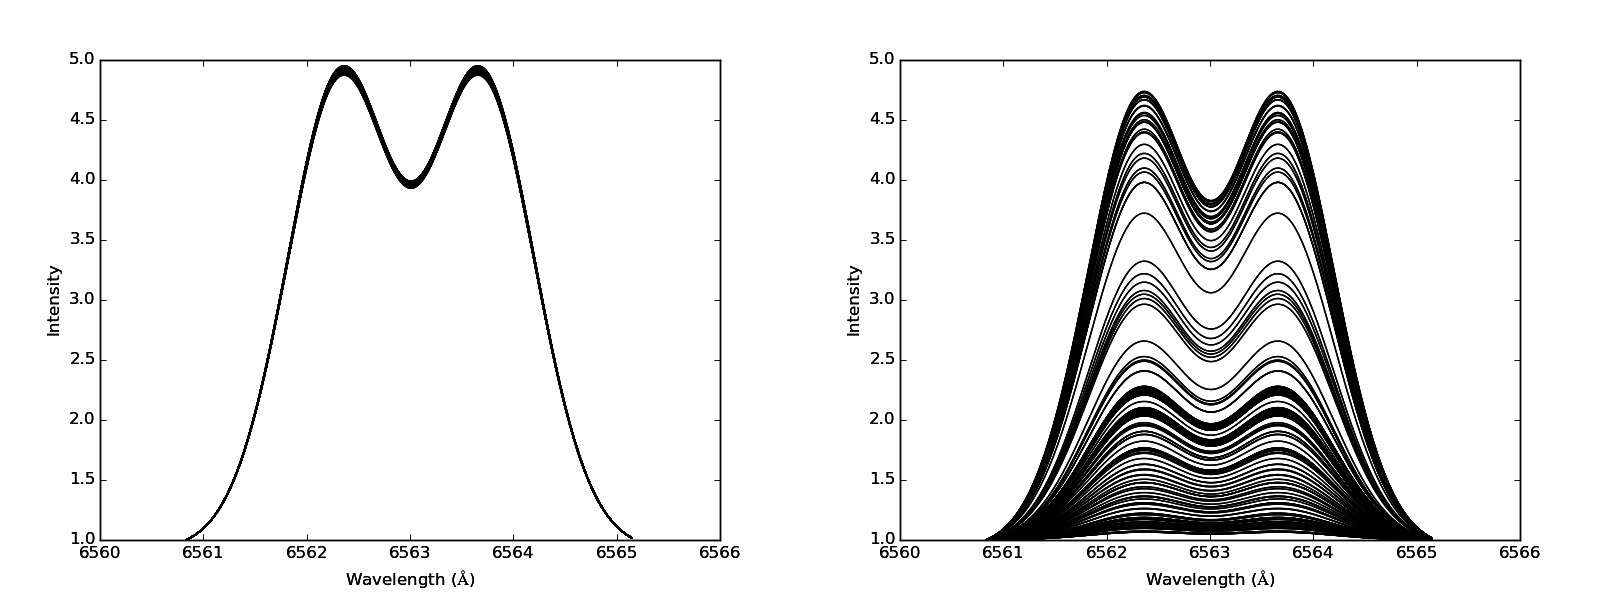
\includegraphics[scale=0.25]{Figures/extremes.png} \\
\end{center}
\caption{This illustrates the effects of extremes of symmetry of plage data on the variations in equivalent width. In
  each case a rotation period of 80 days and a stellar inclination of 90{\degree} is used. In the case on the left 100 plage
  points are distributed randomly over the face of the star whilst in the case on the right the same number of plage
  points are distributed over a 30{\degree} longitude band on one face of the star. The times from the {\harps} data are
  used in the model and all the generated spectra superimposed.} 
\protect\label{fig:extremew}
\end{figure}

Here are presented in table \ref{table:modelcomp} a selection of typical results showing means and standard deviations
for the Equivalent Width method (EW)) with the two plage distributions for various periods and with 30{\degree},
60{\degree} and 90{\degree} inclinations and for 70, 80 and 90-day periods with 10{\degree} to 90{\degree} inclinations.
Note that the PR results are not displayed as variations were insufficient to be displayed in less than 6 figures, the
Doppler variations are just not substantial enough.

\begin{table}[!htbp]
\centering
\scalebox{0.50}{
\begin{tabular}{|l|c|l|l|l|}
\hline
Plage Dist & Period & \multicolumn{1}{|c|}{30\degree}&\multicolumn{1}{|c|}{60\degree}&\multicolumn{1}{|c|}{90\degree}\\\hline
\multirow{8}{*}{Random to 2.5\%} & 20 & 2.150 $ \pm $ 0.572 & 2.746 $ \pm $ 0.939 & 2.735 $ \pm $ 0.891  \\
& 30 &  2.725 $ \pm $ 0.495 & 3.870 $ \pm $ 0.895 &  4.004 $ \pm $ 0.942 \\
& 40 &  1.917 $ \pm $ 0.541 & 2.501 $ \pm $ 0.927 &  2.614 $ \pm $ 0.967 \\
& 50 &  1.604 $ \pm $ 0.483 & 1.996 $ \pm $ 0.805 &  2.018 $ \pm $ 0.876 \\
& 60 &  1.626 $ \pm $ 0.573 & 2.057 $ \pm $ 0.951 &  2.099 $ \pm $ 1.006 \\
& 70 &  1.967 $ \pm $ 0.445 & 2.334 $ \pm $ 0.803 &  2.340 $ \pm $ 0.821 \\
& 80 &  1.637 $ \pm $ 0.495 & 2.161 $ \pm $ 0.805 &  2.309 $ \pm $ 0.828 \\
& 90 &  2.475 $ \pm $ 0.548 & 3.365 $ \pm $ 0.894 &  3.410 $ \pm $ 0.901 \\\hline
\end{tabular}}

\vspace{5 mm}

\scalebox{0.50}{
\begin{tabular}{|l|c|l|l|l|}
\hline
Plage Dist & Incl\degree & \multicolumn{1}{|c|}{70 days}&\multicolumn{1}{|c|}{80 days}&\multicolumn{1}{|c|}{90 days}\\\hline
\multirow{9}{*}{Random to 2.5\%} & 10 & 1.693 $ \pm $ 0.140 & 1.484 $ \pm $ 0.182 & 1.816 $ \pm $ 0.196 \\
& 20 &  1.811 $ \pm $ 0.292 &  1.492 $ \pm $ 0.356 &  2.116 $ \pm $ 0.387 \\
& 30 &  1.967 $ \pm $ 0.445 &  1.637 $ \pm $ 0.495 &  2.475 $ \pm $ 0.548 \\
& 40 &  2.116 $ \pm $ 0.590 &  1.810 $ \pm $ 0.626 &  2.827 $ \pm $ 0.691 \\
& 50 &  2.237 $ \pm $ 0.711 &  1.994 $ \pm $ 0.732 &  3.139 $ \pm $ 0.815 \\
& 60 &  2.334 $ \pm $ 0.803 &  2.161 $ \pm $ 0.805 &  3.365 $ \pm $ 0.894 \\
& 70 &  2.392 $ \pm $ 0.860 &  2.277 $ \pm $ 0.848 &  3.477 $ \pm $ 0.930 \\
& 80 &  2.396 $ \pm $ 0.877 &  2.338 $ \pm $ 0.850 &  3.464 $ \pm $ 0.911 \\
& 90 &  2.340 $ \pm $ 0.821 &  2.309 $ \pm $ 0.828 &  3.410 $ \pm $ 0.901 \\\hline
\end{tabular}}
\caption{Simulated mean equivalent widths with associated standard deviations from simulations for the 2.7\%
  plage distributions and a set of rotation periods and inclinations. In the first table results are illustrated for
  various periods and for 30{\degree}, 60{\degree} and  90{\degree} inclinations. In the second table results are
  illustrated for various inclinations and 70, 80 and 90-day periods as these are close to the
  rotation period of \prox.}
\protect\label{table:modelcomp}
\end{table}

For each set of generated spectra for both plage distributions, rotation period (between 15 and 90 days in steps of 5
and inclination (between 10{\degree} and 90{\degree} in steps of 5\degree), a periodogram was obtained, viewing periods
between 10 days and 130 days in steps of 0.01 days, from the calculated equivalent widths and noted the RMS error over
all inclinations. In nearly all cases the error was rarely more than 0.02 days. It was rather a different matter for the
Peak Ratios however, in that the variations observed in the Peak Ratios were typically $2{\times}10^{-5}$ at most or with
the most extreme plage distributions could be stretched to $2{\times}10^{-4}$. These variations are just above the level
at which it is possible to reliably measure the Peak Ratio from the observed data but far below the observed Peak Ratio
changes in the data which are two orders of magnitude higher, e.g. combining all the {\harps} data, a result of 0.997 $
\pm $ 0.018 (one $\sigma$) was obtained.

\section{Adding in noise and flares}
\protect\label{section:addflares}

Despite the limitations of the simplistic model, it is clear that a good estimate of periodicity may be obtained from
the Equivalent Width method, although the Peak Ratio variations could not be reproduced and that method reliably applied.
These results are for a noiseless set of models and to compare with reality the performance of the modelling results and
the analysis methods in the presence of observational noise and also the influence of simulated flare events has to be
considered.

As a first step in moving to something like actual observational data, noise of a given signal to noise ratio was added
to the simulated spectra and the effect observed on the accuracy of the periodicity measurements for various levels,
inclinations and starting periods. Adding Gaussian noise with SNRs from 40 down to 1 in steps of 0.1 was tried.
These were tried with all the combinations of inclinations and starting periods tried before.

It was noticeable that doing this only started to have any significant effect with SNR below 20. Below this level, two
things started to happen, increasingly as the SNR was reduced. Either the error in the recovered period increased,
although not by very much, alternatively the recovered period was manifestly incorrect, giving a clear False Positive
such as returning a period of 50 days from a starting period of 80 days.

It was easy to discriminate between these two cases by setting a threshold of 5\% for the difference between the
recovered period and the starting period. If the difference exceeded this, then the period was regarded as incorrectly
recovered, otherwise it was regarded as correctly recovered but with the given error. However in all the cases the
difference was either substantially greater or substantially less than this. It was noticeable that in quite a number of
cases a period close to 116 days was returned as a False Positive.

Also examined was the possible effect of flares. The effect of flares was simulated by taking the spectra
which were clipped as having excessive Equivalent Width in Section \ref{section:harpsper}\footnote{N.B. This was done
  with the Original Set of data and observation times as previously noted.} and adding in the same
proportionate excess over the median Equivalent Width in the model as was found in the observed data. The result was a
poorer performance than with noise alone, but not by much. With just noise, the performance became markedly low with a
SNR of 15 or below but adding flares as described significantly reduced the performance with a SNR of 20 or below. These
values of SNR are much lower than the published values for {\uves} and {\harps}, which are in both cases well over
200\footnote{The calculations of Equivalent Width, {\ha} Index and Peak Ratios for {\harps} also calculated the
  uncertainty in the these values, which remained of the same order.}. In Fig. \ref{fig:noiseresults} is illustrated the
effects of adding noise at various levels to the percentage of correct recoveries with either the largest 4 flares
listed in Section \ref{section:uvesflares}, or the ones clipped as having an Equivalent Width greater than 3.8 (one
standard deviation above the median).

In Fig. \ref{fig:noiseresults} is shown the effect of varying SNR and adding in simulated flare data on the rate of
recovery of the correct period. The blue plot shows the effect of just adding noise, the green that of adding in the
four largest flares and noise and the red shows the effect of adding simulated flares from all the values in the
{\harps} data clipped having Equivalent Width over 3.8.

\Notnow{
\begin{table}[!htbp]
\centering
\scalebox{0.75}{
\begin{tabular}{|l|r|r|r|l|r|r|r|}
\hline
SNR & None & Peak 1 & Peaks 1-3 & SNR & None & Peak 1 & Peaks 1-3 \\\hline
25 & 99.50 & 99.00 & 98.40 & 10 & 97.20 & 96.20 & 93.80 \\\hline
20 & 99.50 & 98.80 & 97.90 & 9 & 95.30 & 93.40 & 90.80 \\\hline
19 & 99.30 & 99.10 & 98.30 & 8 & 94.60 & 91.00 & 87.90 \\\hline
18 & 99.30 & 98.80 & 98.10 & 7 & 93.80 & 88.90 & 83.00 \\\hline
17 & 98.60 & 98.30 & 98.10 & 6 & 90.50 & 84.30 & 78.70 \\\hline
16 & 99.50 & 99.00 & 97.90 & 5 & 88.90 & 82.50 & 78.50 \\\hline
15 & 99.70 & 98.60 & 97.90 & 4 & 86.90 & 79.80 & 72.70 \\\hline
14 & 99.00 & 98.80 & 97.20 & 3 & 82.40 & 72.00 & 63.70 \\\hline
13 & 99.00 & 97.40 & 96.50 & 2 & 80.60 & 66.40 & 60.40 \\\hline
12 & 98.40 & 98.10 & 96.40 & 1 & 73.70 & 58.00 & 52.20 \\\hline
1 & 97.10 & 95.30 & 94.10 & 0 & 69.70 & 54.80 & 45.50 \\\hline
\end{tabular}}
\caption{Percentage recovery with integer values of SNR for all inclinations, all starting periods and no flare, just
  largest flare and all the flares for {\harps} discussed in Fig. \ref{fig:proxhists}. Note that this table involves extensive use
  of randomly-generated values for plage distribution and noise and is not exactly reproducible.}
\protect\label{table:noiseresults}
\end{table}}

\begin{figure}[!htbp]
\begin{center}
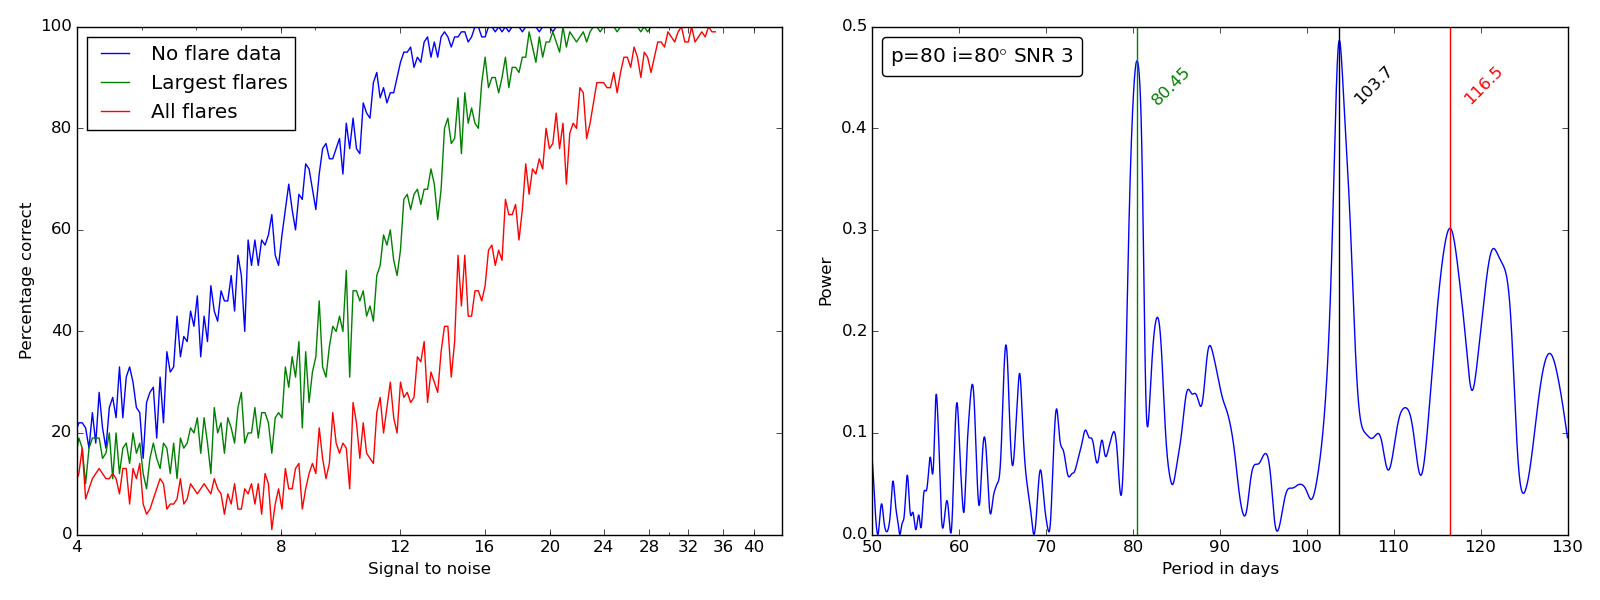
\includegraphics[scale=0.25]{Figures/missedperiod.png} \\
\end{center}
\caption{This figure shows the percent of correctly recovered periods up to 3\% for all periods and inclinations
  with noise added with SNR between 1 to 10 with no flare data added (blue), just the four largest flare data (green)
  and the flare data clipped in Section \ref{section:harpsper} as having Equivalent Width greater than 1 standard
  deviation from the median.}
\protect\label{fig:noiseresults}
\end{figure}
